\documentclass[11pt,reqno]{amsart}
\usepackage[margin=1.15in]{geometry}
\usepackage{amsmath,amssymb,amsthm,mathtools}
\usepackage{graphicx}
\usepackage{booktabs}
\usepackage[colorlinks=true,linkcolor=blue,citecolor=blue,urlcolor=blue]{hyperref}
\usepackage{microtype}
\usepackage{xurl}
\raggedbottom

\theoremstyle{plain}
\newtheorem{theorem}{Theorem}
\newtheorem{proposition}[theorem]{Proposition}
\newtheorem{corollary}[theorem]{Corollary}
\newtheorem{lemma}[theorem]{Lemma}
\theoremstyle{definition}
\newtheorem{definition}[theorem]{Definition}
\newtheorem{remark}[theorem]{Remark}
\newtheorem{observation}[theorem]{Observation}

\DeclareMathOperator{\sqf}{sqf}
\newcommand{\Art}{\mathrm{A}}
\newcommand{\E}{\mathbb{E}}
\newcommand{\Leg}[2]{\left(\frac{#1}{#2}\right)}
\newcommand{\Z}{\mathbb{Z}}
\newcommand{\Q}{\mathbb{Q}}

\begin{document}

\title[Quadratic exclusion laws for consecutive Artin primes]
{Quadratic exclusion laws for consecutive Artin primes in arbitrary bases}

\author{Josh Bald}
\address{Ontario, Canada}
\email{jpbald93@gmail.com}

\subjclass[2020]{Primary 11A07; Secondary 11N05, 11N13, 11Y16, 11Y60}
\keywords{Artin's conjecture, primitive roots, consecutive primes, quadratic
characters, prime discriminants, Lemke Oliver--Soundararajan bias}

\date{September 10, 2026}

\begin{abstract}
Let $a \ge 2$ be a non-square integer with squarefree part $d$, and say that
an odd prime $p$ is \emph{Artin base $a$} if $a$ is a primitive root
modulo $p$. (We restrict to odd primes throughout: modulo $2$ every odd
integer trivially has full multiplicative order, and the quadratic obstruction
below fails there.) Membership in $\Art_a$ forces the quadratic character value
$\chi_a(p) = -1$, and since $\chi_a$ has conductor $f$, this necessary
condition depends only on $p \bmod f$. We determine, for every non-square base
$a$, the exact set of gap classes on which the resulting \emph{quadratic
obstruction} forbids two primes from both being Artin base $a$. The forbidden
classes themselves are not new: Tinkov\'a, Waxman and
Zindulka~\cite{TinkovaWaxmanZindulka2023}, studying Artin prime pairs at a
fixed even shift, gave sufficient conditions on $(d, g)$ for the pair set to
be empty, and we have verified that their conditions and our classification
agree on every non-square base $a \le 80$, the exceptional squarefree part
$d = 5$ included. Our contribution to the classification is therefore one of
method and of completeness rather than of discovery: we derive the classes
from an exact counting identity, obtain the converse direction --- that
outside the listed cases \emph{no} quadratic exclusion class exists --- as a
theorem rather than a conjecture, cover bases excluded from their hypothesis
$g \in \mathcal{H}_1$ (perfect powers such as $a = 8, 27, 32$), and
machine-check the key steps in Lean~4. Two mechanisms
produce such \emph{exclusion classes}. The first is \emph{reversal}:
$\chi_a(q) = -\chi_a(p)$ for all admissible $p, q = p + g$, so one of the two
primes is a quadratic residue base $a$; we classify the reversing classes
completely via the factorization of the discriminant of $\Q(\sqrt{a})$ into
prime discriminants. The second, operating when no reversing class exists, is
\emph{inadmissibility}. Its analysis rests on an exact count, and we prove the
general identity
$4 N_{--}(g) = T(g) - A(g) - B(g) + S(g)$
valid for every modulus, prime or composite, from which the prime-conductor
evaluation $N_{--}(g) = (d - 3 + 2\chi(g))/4$ for $g \not\equiv 0 \pmod d$ (and
$N_{--}(0) = (d-1)/2$) follows as a special case. The resulting complete
dichotomy is: base $a$ admits a quadratic exclusion class if and only if $d$ is
even, $d \equiv 3 \pmod 4$, $3 \mid d$, or $d = 5$. We emphasise throughout
that the quadratic obstruction is \emph{necessary but not sufficient} for
Artin status, so an exclusion class is a proof of impossibility, while the
absence of one is not a proof of possibility. The classification is verified
by exhaustive computation for all non-square $2 \le a \le 80$, and the
exclusion laws hold without exception across $84{,}981{,}870$ base--pair
incidences below $10^9$. The counting identity, together with the
$d = 5$ and $d = 13$ cases of the prime-conductor count, is additionally
machine-checked in Lean~4.

We then measure, for eleven bases, the consecutive-pair Artin correlation
$\delta(a)$ over all $50{,}847{,}531$ consecutive prime pairs below $10^9$
with smaller member at least $5$. The exclusion weight $w$ correlates with $|\delta|$ at $r = 0.646$, but this
association is confounded with the conductor: $r(\log f, |\delta|) = -0.957$,
the partial correlation of $w$ given $\log f$ is only $0.136$, and the three
bases with no exclusion classes still carry $|\delta|$ up to $0.043$.
Restricting $\delta$ to gap classes outside the exclusion set yields a
positive value for all eight bases that possess such classes. Among the
quantities compared, the conductor of $\chi_a$ is the stronger descriptive
predictor of the global correlation; we do not claim it is the operative
mechanism.
\end{abstract}

\maketitle

\section{Introduction}
\label{sec:intro}

Artin's conjecture on primitive roots asserts that for a non-square integer
$a \neq -1$ the set of primes $p$ for which $a$ is a primitive root modulo $p$
has a positive density, given by an explicit rational multiple of Artin's
constant. It is known under GRH by Hooley~\cite{Hooley1967}. Unconditionally, and for the weaker assertion of infinitude rather than
positive density, Heath-Brown~\cite{HeathBrown1986}, building on
Gupta--Murty~\cite{GuptaMurty1984}, proved that all but at most two prime
bases are primitive roots for infinitely many primes; in particular, of any
three distinct primes, at least one is a primitive root for infinitely many
$p$. This infinitude statement should be kept separate from Hooley's
conditional density theorem. See Moree's survey~\cite{Moree2012} for the extensive
literature, and \cite{FanPollack2025, PeruccaShparlinski2025} for recent
uniform versions.

Write
\[
  \Art_a = \{\, p \text{ an odd prime} : a \text{ is a primitive root mod } p \,\},
\]
and call $p \in \Art_a$ an \emph{Artin prime base $a$}. The restriction to odd
primes is not cosmetic. Modulo $2$ the group $(\Z/2\Z)^\times$ is trivial, so
every odd $a$ vacuously has full order, while $\chi_a(2)$ need not be $-1$;
taking $a = 33$, the primes $2$ and $13$ both have $33$ as a primitive root
even though their gap $11$ lies in a reversing class modulo the conductor
$33$. Every statement below therefore concerns odd primes only, as the
hypotheses of Lemma~\ref{lem:obstruction} and Theorem~\ref{thm:exclusion}
already record. Recent work continues in the same single-prime direction: J\"arviniemi,
Perucca and Sgobba~\cite{JarviniemiPeruccaSgobba2025} give a unified treatment
of Artin-type density problems, and Kimmel~\cite{Kimmel2024} treats Artin's
conjecture in number fields and for matrices; the Artin-density conclusions in
both are conditional on GRH. All results above
concern a \emph{single} prime at a time. The behaviour of Artin primes in
\emph{pairs} has been studied much less. Garcia, Kahoro and
Luca~\cite{GarciaKahoroLuca2019} (see also~\cite{GarciaLucaShiUdell2020})
investigated primitive-root bias for twin primes; Pollack~\cite{Pollack2014}
showed under GRH that for a fixed admissible base there are infinitely many
bounded-gap runs of primes all having that base as a primitive root;
Baker--Pollack~\cite{BakerPollack2016} proved unconditionally that there are
strings of consecutive primes each having \emph{some} primitive root from a
large prescribed set, where the root may depend on the prime. Closest to the
present work, Tinkov\'a, Waxman and Zindulka~\cite{TinkovaWaxmanZindulka2023}
model the count of Artin prime pairs at a fixed even shift and, as part of
that analysis, identify shift--base pairs for which the count vanishes
identically; their vanishing conditions coincide with the classification
obtained here, and Section~\ref{sec:twz} sets out the overlap in detail.

The starting point of this paper is an elementary observation, made
independently here and by Tinkov\'a, Waxman and
Zindulka~\cite{TinkovaWaxmanZindulka2023} (see the comparison in
Section~\ref{sec:twz}). Since a quadratic residue cannot generate the cyclic group
$(\Z/p\Z)^\times$ of even order $p - 1$, membership in $\Art_a$ forces
$\chi_a(p) = -1$, where $\chi_a$ is the quadratic character attached to
$\Q(\sqrt{a})$. Because $\chi_a$ is a character modulo the conductor $f$ of
that field, the value $\chi_a(p)$ depends only on $p \bmod f$. Consequently, if
a shift $g$ has the property that it \emph{reverses} $\chi_a$ on every
admissible residue class modulo $f$, then for any two primes $p$ and $q = p+g'$
with $g' \equiv g \pmod f$, \emph{neither dividing $a$}, we get
$\chi_a(q) = -\chi_a(p)$, so at least one of $\chi_a(p), \chi_a(q)$ equals
$+1$ --- and that prime is not Artin base $a$. A prime dividing $a$ is not
Artin base $a$ either, since then $a$ is not even a unit; so two odd primes at
such a gap can never \emph{both} be Artin base $a$. We call this
a \emph{quadratic exclusion law} (Theorem~\ref{thm:exclusion}).

\subsection*{What this paper does and does not classify}
It is essential to be precise about the scope of the classification, and we
state the limitation once, plainly, so that no result below is read as more
than it is. The condition $\chi_a(p) = -1$ is \emph{necessary} for $p \in
\Art_a$ but far from \emph{sufficient}: $a$ must also be a non-$\ell$-th-power
residue modulo $p$ for every odd prime $\ell \mid p-1$. What we classify
completely is the set of gap classes on which the \emph{quadratic} obstruction
alone forbids a doubly-Artin pair (Definition~\ref{def:exclusion}). Therefore:

\begin{itemize}
\item when a gap class \emph{is} a quadratic exclusion class, no pair of
      \emph{odd} primes at that gap can both be Artin base $a$ --- an
      unconditional theorem;
\item when a gap class is \emph{not} a quadratic exclusion class, we conclude
      nothing. Higher-order obstructions may still forbid doubly-Artin pairs
      there, and our results do not assert that such pairs exist.
\end{itemize}

Accordingly, ``base $a$ admits no exclusion class'' below always abbreviates
``base $a$ admits no \emph{quadratic} exclusion class''. Establishing that
doubly-Artin pairs actually occur at the remaining gaps is a different and
harder problem, of the type addressed under GRH in~\cite{Pollack2014}; we do
not address it. The empirical sections confirm that doubly-Artin pairs are
abundant outside the exclusion classes; such observations do establish
existence for the configurations actually exhibited, but abundance in a finite
range is neither an infinitude theorem nor an existence theorem for every
remaining gap class.

\subsection*{Relation to Tinkov\'a--Waxman--Zindulka}
\label{sec:twz}

The forbidden gap classes classified here have been obtained before, by a
different route, and we state the overlap precisely before describing what
this paper adds.

Tinkov\'a, Waxman and Zindulka~\cite{TinkovaWaxmanZindulka2023} study Artin
prime pairs: for a fixed even shift $d$ and a base $g$, they consider the set
$\pi_{d,g}$ of primes $p$ such that $g$ is a primitive root modulo both $p$
and $p + d$. They observe, exactly as we do, that $p \in \mathcal{P}_g$ forces
$\Leg{g}{p} = -1$, and they identify pairs $(d,g)$ for which the resulting
quadratic condition cannot be met by both members, so that $\pi_{d,g}$ is
empty. Their Theorem~1.1 lists these cases: with $g = g_0 g_s^2$ and $g_0$
squarefree, $\pi_{d,g}$ is empty if $g_0 = 5$ and $d \equiv 2, 3 \pmod 5$; or
if $g_0 \mid d$ with $(d \equiv 2 \bmod 4,\ g_0 \equiv 3 \bmod 4)$ or
$(d \equiv 4 \bmod 8,\ g_0 \equiv 2 \bmod 4)$; or if $g_0 \nmid d$,
$g_0 \mid 3d$, and one of three further congruence conditions holds.

Translating their $(d, g_0)$ into our $(g, d)$ --- their shift is our gap and
their squarefree part is ours --- their conditions and our classification
select the same bases. We checked this over all $72$ non-square
$a \le 80$: the set of bases admitting some forbidden gap agrees in every
case, including the exceptional squarefree part $d = 5$, which we reach
through the inadmissibility mechanism of Theorem~\ref{thm:inadmissible} and
they reach through their condition~(1). We claim no priority for the
classification itself, and an earlier version of this paper, which described
the classes as apparently unrecorded, was wrong to do so.

What this paper adds to the classification is the following.
\begin{itemize}
\item \emph{A converse.} Their Theorem~1.1 gives sufficient conditions for
      emptiness and conjectures that $\pi_{d,g}$ is infinite otherwise. We
      prove the converse at the level of the quadratic obstruction: outside
      the listed cases, no quadratic exclusion class exists
      (Corollary~\ref{cor:complete} and Proposition~\ref{prop:exhaustion}).
      This is a weaker statement than their conjecture --- it does not assert
      that doubly-Artin pairs occur --- but it is a theorem.
\item \emph{A different derivation.} We obtain the classes from the exact
      counting identity of Theorem~\ref{thm:identity}, valid for every
      modulus, prime or composite, rather than from a case analysis of
      quadratic reciprocity. The identity yields the prime-conductor
      evaluation $N_{--}(g) = (d - 3 + 2\chi(g))/4$ as a special case.
\item \emph{Bases they exclude.} Their hypothesis $g \in \mathcal{H}_1$
      omits perfect powers; among non-square $a \le 80$ this omits
      $a = 8, 27, 32$. Our classification depends only on the squarefree part
      and covers them.
\item \emph{Machine verification.} The counting identity and the $d = 5$ and
      $d = 13$ cases are checked in Lean~4 (Section~\ref{sec:formal}).
\item \emph{Consecutive rather than fixed-shift pairs, and a census.} Their
      pairs $(p, p+d)$ need not be consecutive. Sections
      \ref{sec:verification}--\ref{sec:delta} concern consecutive primes and
      the cross-base correlation $\delta(a)$, which is independent of the
      classification and which we believe to be new.
\end{itemize}

We record the remainder of our literature search, which located no other
statement of this kind. Moree's hundred-page
survey~\cite{Moree2012} uses the quadratic obstruction $\chi_a(p) = -1$
throughout --- it is the source of the entanglement correction in Hooley's
density --- but always as a condition on a \emph{single} prime; shifts of the
argument of $\chi_a$, and the resulting constraints on \emph{pairs} of primes,
do not appear. Garcia--Kahoro--Luca~\cite{GarciaKahoroLuca2019} and its
sequel~\cite{GarciaLucaShiUdell2020} concern the single gap $g = 2$ and a
different statistic --- a bias between the twin-prime components in the
\emph{number} of primitive roots, $\varphi(p-1)$ versus $\varphi(p+1)$ --- not
the joint Artin status of the pair; the reversing mechanism plays no role
there. Pollack~\cite{Pollack2014} produces, under GRH, bounded-gap runs of primes
sharing one fixed primitive root, and
Baker--Pollack~\cite{BakerPollack2016} obtain unconditionally strings of
consecutive primes each of which has \emph{some} primitive root drawn from a
large prescribed set of primes --- the root being allowed to vary with the
prime. Neither of these two imposes structure on the gap classes, and neither
identifies forbidden ones; the forbidden classes are identified
in~\cite{TinkovaWaxmanZindulka2023}, as described above. We likewise searched
for forbidden-gap statements for quadratic characters in other contexts ---
consecutive quadratic residues and non-residues have a classical literature
--- and found constraints on character values along progressions, but no
further statement coupling a gap \emph{class} to the joint primitive-root
status of a pair of primes. We note that our own search initially missed
\cite{TinkovaWaxmanZindulka2023}, whose notation names the shift $d$ and the
base $g$, reversing the roles those letters play here; the omission was caught
in adversarial review.

The reversing classes are determined by the following theorem; combined with
the exhaustion proposition (Proposition~\ref{prop:exhaustion}) and the
inadmissibility count (Theorem~\ref{thm:inadmissible}), which supplies the
exceptional case $d = 5$, this determines the full set of quadratic exclusion
classes for every base.

\begin{theorem}[Classification of reversing classes; see
Theorem~\ref{thm:classification}]
Let $a$ be a non-square positive integer with squarefree part $d$, let $D$ be
the discriminant of $\Q(\sqrt{d})$, and factor $D = D_1 D_2 \cdots D_k$ into
prime discriminants. Then an even shift $g$ is a reversing class for base $a$
if and only if no component $D_i$ is \emph{indeterminate} at $g$ and an odd
number of the components \emph{reverse} at $g$, where the behaviour of each
component is given by Table~\ref{tab:components}.
\end{theorem}

Reversal is not the only route to exclusion. Exclusion of doubly-Artin pairs
at a gap class requires only that \emph{no admissible residue} $r$ have
$\chi_a(r) = \chi_a(r+g) = -1$; reversal is the generic way this happens, but
it can also happen because the offending configurations are ruled out by
admissibility, i.e.\ they would force $p$ or $p+g$ to be divisible by an odd
prime factor of the conductor. Analysing this second mechanism requires an
exact count of the doubly-negative residues, and the engine of the paper is
the following identity, which holds for every modulus and requires no
primality hypothesis whatever.

\begin{theorem}[Counting identity; see Theorem~\ref{thm:identity}]
Let $\chi$ be a real character modulo $m$ taking values in $\{0, \pm 1\}$, let
$g$ be a shift, and set
$U(g) = \{ r \bmod m : \chi(r) \neq 0,\ \chi(r+g) \neq 0 \}$,
$T(g) = |U(g)|$, $A(g) = \sum_{r \in U(g)} \chi(r)$,
$B(g) = \sum_{r \in U(g)} \chi(r+g)$,
$S(g) = \sum_{r \in U(g)} \chi(r)\chi(r+g)$. Then
\[
  4\, N_{--}(g) \;=\; T(g) - A(g) - B(g) + S(g),
  \qquad
  N_{--}(g) = \#\{\, r \in U(g) : \chi(r) = \chi(r+g) = -1 \,\}.
\]
\end{theorem}

Specialising to prime conductor recovers a closed form, and it is here that a
hypothesis is genuinely needed.

\begin{theorem}[Inadmissibility exclusion; see Theorem~\ref{thm:inadmissible}]
Let $d \equiv 1 \pmod 4$ be a prime, so that $\chi_a$ for $\sqf(a) = d$ has
odd conductor $d$ and no reversing classes exist. For $g \not\equiv 0 \pmod d$
the number of residues $r \bmod d$ with $r, r+g \not\equiv 0$ and
$\chi(r) = \chi(r+g) = -1$ equals $\bigl(d - 3 + 2\chi(g)\bigr)/4$, while
$N_{--}(0) = (d-1)/2$. The count vanishes if and only if $d = 5$ and
$\chi(g) = -1$, i.e.\ $g \equiv 2, 3 \pmod 5$. Consequently base $5$ (and any
$a$ with $\sqf(a) = 5$) admits the exclusion classes $g \equiv 2, 3 \pmod 5$,
while for prime $d \equiv 1 \pmod 4$ with $d \ge 13$ no exclusion class
exists. (Empirically these two classes contain $40.4\%$ of the consecutive
prime pairs in our census, i.e.\ those with smaller member at least $5$ and
larger member below $10^9$; that is a measured proportion, not part of the
theorem.)
\end{theorem}

The hypothesis $g \not\equiv 0 \pmod d$ is not cosmetic. Since $\chi(0) = 0$,
evaluating the displayed formula at $g \equiv 0$ would give
$(d - 3 + 2\chi(0))/4 = (d-3)/4$, which is not in general an integer --- for
$d = 13$ it gives $2.5$ against a true count of $6$ --- so the $g \equiv 0$
case must be handled separately, as it is above. Both branches of the count
are machine-checked for $d = 5$ and $d = 13$ (Section~\ref{sec:formal}).

The classification is sharp enough to answer the qualitative question
completely.

\begin{corollary}[Complete dichotomy; see Corollary~\ref{cor:complete}]
Base $a$ admits at least one quadratic exclusion class if and only if $d$ is
even, or $d \equiv 3 \pmod 4$, or $3 \mid d$ (these give reversing classes), or
$d = 5$ (inadmissibility classes).
\end{corollary}

Thus for $d \in \{13, 17, 29, 37, 41, 53, 61, \dots\}$ there is no quadratic
exclusion law at all, while for $d = 3$ fully half of the even gap classes
modulo $12$ are exclusion classes, and for $d = 5$ two of the five
gap classes modulo $5$ are excluded. The reversing dichotomy is a genuine
structural phenomenon whose source is a degeneration of a Jacobi-sum
obstruction at the single prime $3$ (Remark~\ref{rem:three}); the
inadmissibility phenomenon is a second, independent degeneration, this time of
a counting bound at the single prime $5$
(Theorem~\ref{thm:inadmissible}).

In the second half of the paper we turn from the deterministic statement to a
statistical one. For a base $a$ define the consecutive-pair correlation
\begin{equation}
\label{eq:delta}
  \delta(a) \;=\; P\bigl(p_{n+1} \in \Art_a \mid p_n \in \Art_a\bigr)
             \;-\; P\bigl(p_{n+1} \in \Art_a \mid p_n \notin \Art_a\bigr),
\end{equation}
computed over consecutive primes $p_n < p_{n+1} \le x$. The bias of
Lemke Oliver and Soundararajan~\cite{LOS2016} in the joint distribution of
$(p_n \bmod m, p_{n+1} \bmod m)$ may propagate, through the factorization of
$p - 1$, into Artin status, so one expects $\delta(a) \neq 0$; and indeed we
find $\delta(a) < 0$ for all eleven bases examined.

The natural guess is that the exclusion laws drive this anticorrelation: bases
whose exclusion classes capture a larger share of consecutive pairs should
display a more negative $\delta$. The data complicate this guess in an
instructive way. Over all $50{,}847{,}531$ consecutive prime pairs below
$10^9$ we find

\begin{itemize}
\item the raw association is substantial, $r(w, |\delta|) = 0.646$ over the
      eleven bases, where $w$ is the weighted fraction of pairs in exclusion
      classes --- but it is confounded with the conductor, since large $w$
      occurs only at small $f$: $r(w, \log f) = -0.643$, and the partial
      correlation of $w$ with $|\delta|$ given $\log f$ collapses to $0.136$;
\item the three bases with no exclusion classes at all ($a = 13, 17, 29$)
      still exhibit $|\delta|$ from $0.022$ to $0.043$; base $13$ alone exceeds
      seven of the other ten bases (bases $13, 17, 29$ rank fourth, sixth and
      eighth of eleven), so exclusion structure is not necessary for strong
      anticorrelation;
\item $r(\log f, |\delta|) = -0.957$: conductor size orders the data far
      better than exclusion weight does;
\item restricting $\delta$ to gap classes outside the exclusion set
      (Table~\ref{tab:outside}) gives a \emph{positive} value for all eight
      bases possessing such classes --- a sign reversal under restriction,
      which is not an additive decomposition of the global value.
\end{itemize}

A possible explanation --- which we propose rather than establish --- is that
the residue information relevant to $\chi_a$ is carried by the $\varphi(f)$
classes modulo $f$, so that the smaller the conductor, the fewer the channels
over which the Lemke Oliver--Soundararajan transition bias is distributed, and
the less cancellation between them. We state the association itself as a
measured empirical regularity (Observation~\ref{obs:conductor}) rather than a
conjectured exact power of $f$, because the data do not support a clean
exponent, and we do not claim the channel count is the operative mechanism.

\subsection*{A note on inferential language}
The computation reported here is an exhaustive census of a finite set: every
prime below $10^9$ is examined, and every count is exact. There is no
sampling. We therefore avoid the vocabulary of statistical inference in
describing the results. Where a $z$-score appears in Table~\ref{tab:delta} it
is a nominal, descriptive scale factor computed under a binomial reference
model that is certainly false here --- consecutive pairs overlap, and the
population is deterministic --- and it should be read only as the ratio of the
effect to that reference scale, not as a test of any hypothesis. For
definiteness, with $n_{ij}$ as in Section~\ref{sec:delta}, write
$r_A = n_{10} + n_{11}$, $r_N = n_{00} + n_{01}$,
$\widehat{p}_{A} = n_{11}/r_A$ and $\widehat{p}_{N} = n_{01}/r_N$; then
\[
  z = \frac{\widehat{p}_A - \widehat{p}_N}{s},
  \qquad
  s = \sqrt{\frac{\widehat{p}_A(1 - \widehat{p}_A)}{r_A}
           + \frac{\widehat{p}_N(1 - \widehat{p}_N)}{r_N}}\,,
\]
that is, separate fitted proportions rather than a pooled one, and no
continuity correction. The precision
of the quoted digits of $\delta$ rests on the counts being exact integers, not
on any $z$-value. Correlations across the eleven bases are descriptive summaries of
eleven points, not estimates from a random sample of bases.

\subsection*{Summary of results}
Section~\ref{sec:exclusion} proves the exclusion law and classifies the
reversing classes. Section~\ref{sec:identity} proves the counting identity and
derives the inadmissibility mechanism and the complete dichotomy.
Section~\ref{sec:formal} describes the machine verification.
Section~\ref{sec:computation} describes the computation.
Section~\ref{sec:verification} reports the verification of the exclusion law at
$10^9$. Section~\ref{sec:delta} reports the measurement of $\delta(a)$, the
failure of exclusion weight to order these data, and the conductor
regularity. Section~\ref{sec:discussion} discusses what we take the
consequences to be.

\section{The exclusion law and the reversing classes}
\label{sec:exclusion}

Throughout, $a \ge 2$ is an integer that is not a perfect square, $d = \sqf(a)$
denotes its squarefree part, and
\begin{equation}
\label{eq:disc}
  D = \begin{cases} d, & d \equiv 1 \pmod 4,\\ 4d, & \text{otherwise,}\end{cases}
  \qquad f = |D|,
\end{equation}
so that $D$ is the discriminant of $K = \Q(\sqrt{a}) = \Q(\sqrt{d})$ and $f$ is
the conductor of the associated quadratic character
$\chi_a = \Leg{D}{\cdot}$. By quadratic reciprocity $\chi_a$ is a Dirichlet
character modulo $f$; in particular
\begin{equation}
\label{eq:modf}
  \chi_a(p) \text{ depends only on } p \bmod f \qquad (p \nmid 2d).
\end{equation}

We recall the elementary obstruction, which is the only number-theoretic input
to Theorem~\ref{thm:exclusion}.

\begin{lemma}
\label{lem:obstruction}
Let $p > 2$ be a prime with $p \nmid a$. If $a$ is a primitive root modulo $p$
then $\chi_a(p) = -1$.
\end{lemma}

\begin{proof}
If $\chi_a(p) = +1$ then $a \equiv b^2 \pmod p$ for some $b$, whence
$a^{(p-1)/2} \equiv b^{p-1} \equiv 1 \pmod p$. Since $p > 2$, $(p-1)/2 < p-1$,
so the multiplicative order of $a$ is a proper divisor of $p - 1$ and $a$ is not
a primitive root.
\end{proof}

The converse fails, and this is the reason for the scope restriction announced
in Section~\ref{sec:intro}: $\chi_a(p) = -1$ does not make $a$ a primitive
root. For instance $\chi_2(43) = -1$, yet $2$ has order $14$ modulo $43$ rather
than the full order $42$.

\begin{definition}
\label{def:shift}
Let $R_f = (\Z/f\Z)^\times$ be the group of reduced residues modulo $f$. (By
Dirichlet's theorem on primes in arithmetic progressions every class in $R_f$
contains infinitely many primes, so nothing is lost by working with all reduced
residues rather than only those realised by primes.) For an even integer $g$,
say that $g$ is
\begin{itemize}
\item \emph{reversing} for $a$ if $\chi_a(r+g) = -\chi_a(r)$ for all $r \in R_f$
      with $r + g \in R_f$;
\item \emph{preserving} for $a$ if $\chi_a(r+g) = +\chi_a(r)$ for all such $r$;
\item \emph{indeterminate} otherwise.
\end{itemize}
\end{definition}

\begin{definition}
\label{def:exclusion}
A class $g \bmod f$ is a \emph{quadratic exclusion class} for base $a$ if it
admits an even representative --- equivalently, any class when $f$ is odd, and
an even class when $f$ is even --- and there is no residue $r \in R_f$ with
$r + g \in R_f$ and $\chi_a(r) = \chi_a(r+g) = -1$. The parity proviso
excludes a trivial case: when $f$ is even, an odd $g$ admits no $r$ with $r$
and $r+g$ both odd, so the defining condition would hold vacuously. Since all
gaps between odd primes are even, nothing of interest is lost. Every reversing class is an exclusion class
(Theorem~\ref{thm:exclusion}); Theorem~\ref{thm:inadmissible} below exhibits
exclusion classes that are not reversing. As stressed in
Section~\ref{sec:intro}, this is a condition on the quadratic character only.
\end{definition}

\begin{theorem}[Quadratic exclusion law]
\label{thm:exclusion}
Let $g$ be reversing for $a$. Then there is no pair of primes $p, q > 2$ with
$p, q \nmid a$, $q - p \equiv g \pmod f$, such that $a$ is a primitive root
modulo both $p$ and $q$.
\end{theorem}

\begin{proof}
By~\eqref{eq:modf} and Definition~\ref{def:shift},
$\chi_a(q) = \chi_a(p + (q-p)) = -\chi_a(p)$. Hence exactly one of
$\chi_a(p), \chi_a(q)$ equals $+1$, and by Lemma~\ref{lem:obstruction} the
corresponding prime is not Artin base $a$.
\end{proof}

Theorem~\ref{thm:exclusion} is unconditional and its proof is three lines; the
content lies in determining the reversing classes, which we now do. Recall that
every fundamental discriminant $D$ factors uniquely as a product of
\emph{prime discriminants}
\begin{equation}
\label{eq:primedisc}
  D = D_1 D_2 \cdots D_k, \qquad
  D_i \in \{-4\} \cup \{8, -8\} \cup \{\, q^* : q \text{ odd prime} \,\},
\end{equation}
where $q^* = q$ if $q \equiv 1 \pmod 4$ and $q^* = -q$ if $q \equiv 3 \pmod 4$
(throughout $\chi_a = \Leg{D}{\cdot}$ is the \emph{Kronecker} symbol, which is
defined at the even arguments occurring for odd conductors, as distinct from
the Legendre symbol $\Leg{\cdot}{q}$ of the component lemma);
the odd $D_i$ are precisely the $q^*$ for the odd primes $q \mid d$, and a
$2$-primary factor $-4$, $8$ or $-8$ occurs according to $d \bmod 8$. Correspondingly
$\chi_a = \prod_i \chi_{D_i}$, with $\chi_{D_i}$ of conductor $|D_i|$.

\begin{table}[t]
\centering
\caption{Behaviour of each prime-discriminant component of $\chi_a$ under the
shift $r \mapsto r + g$. Here $q \ge 5$ is an odd prime.}
\label{tab:components}
\begin{tabular}{llll}
\toprule
component $D_i$ & conductor & reversing iff & preserving iff \\
\midrule
$-4$        & $4$ & $g \equiv 2 \pmod 4$   & $g \equiv 0 \pmod 4$ \\
$8$ or $-8$ & $8$ & $g \equiv 4 \pmod 8$   & $g \equiv 0 \pmod 8$ \\
$-3$        & $3$ & $g \not\equiv 0 \pmod 3$ & $g \equiv 0 \pmod 3$ \\
$q^*$, $q \ge 5$ & $q$ & never             & $g \equiv 0 \pmod q$ \\
\bottomrule
\end{tabular}
\end{table}

\begin{proposition}
\label{prop:components}
Table~\ref{tab:components} is correct: each component behaves as stated, and in
the cases not listed as reversing or preserving it is indeterminate. In
particular a component of conductor $8$ is indeterminate for
$g \equiv 2, 6 \pmod 8$, and a component $q^*$ with $q \ge 5$ is indeterminate
for every $g \not\equiv 0 \pmod q$.
\end{proposition}

\begin{proof}
\emph{Conductor $4$.} $\chi_{-4}(r) = (-1)^{(r-1)/2}$ depends only on
$r \bmod 4$, and on $\{1,3\}$ it is injective. A shift by $g \equiv 2 \pmod 4$
interchanges $1$ and $3$, hence reverses; $g \equiv 0 \pmod 4$ fixes both.

\emph{Conductor $8$.} $\chi_8(r) = +1$ iff $r \equiv \pm 1 \pmod 8$, so the
fibres are $\{1,7\}$ and $\{3,5\}$; the map $r \mapsto r + 4$ interchanges these
two sets, hence reverses, while $r \mapsto r$ preserves. For $g \equiv 2
\pmod 8$ we have $1 \mapsto 3$ (a reversal) but $3 \mapsto 5$ (a preservation),
so the behaviour depends on the class and $g$ is indeterminate; similarly for
$g \equiv 6$. The same computation applies to $\chi_{-8}$, whose $+1$-fibre is
$\{1,3\}$ and whose $-1$-fibre is $\{5,7\}$, again interchanged by $+4$.

\emph{Conductor $3$.} $\chi_{-3}(r) = +1$ iff $r \equiv 1 \pmod 3$. On the two
admissible classes $\{1,2\}$ the character is injective, so any
$g \not\equiv 0 \pmod 3$ moves $1 \leftrightarrow 2$ and reverses, while
$g \equiv 0$ preserves. Note that for a fixed such $g$ only one class $r$
satisfies $r, r+g \not\equiv 0 \pmod 3$, so the uniformity required by
Definition~\ref{def:shift} is a condition on a single residue.

\emph{Conductor $q \ge 5$.} Suppose, for a contradiction, that
$\chi_{q^*}(r+g) = \varepsilon\, \chi_{q^*}(r)$ for a fixed $\varepsilon \in
\{\pm 1\}$, all $r$ with $r, r+g \not\equiv 0 \pmod q$, and some
$g \not\equiv 0 \pmod q$. Multiplying by $\chi_{q^*}(r)$ and summing over
$r \bmod q$ gives
\begin{equation}
\label{eq:jacobi}
  S(g) \;:=\; \sum_{r \bmod q} \chi_{q^*}(r)\,\chi_{q^*}(r+g)
        \;=\; \varepsilon \cdot \#\{\, r : r, r+g \not\equiv 0 \,\}
        \;=\; \varepsilon\,(q-2).
\end{equation}
On the other hand, for $g \not\equiv 0 \pmod q$ the substitution
$r = g t$ (legitimate since $g$ is invertible) and the complete
multiplicativity of $\chi_{q^*}$ give
\[
  S(g) = \sum_{t \bmod q} \chi_{q^*}(gt)\chi_{q^*}(g(t+1))
       = \chi_{q^*}(g)^2 \sum_{t} \chi_{q^*}(t)\chi_{q^*}(t+1)
       = \sum_{t \bmod q} \chi_{q^*}\!\left(\frac{t+1}{t}\right),
\]
the last sum being over $t \not\equiv 0$. As $t$ runs over the nonzero classes,
$u = (t+1)/t = 1 + t^{-1}$ runs over all classes except $u = 1$, whence
\[
  S(g) = \sum_{u \neq 1} \chi_{q^*}(u) = \left(\sum_{u \bmod q} \chi_{q^*}(u)\right) - \chi_{q^*}(1) = 0 - 1 = -1 .
\]
Comparing with~\eqref{eq:jacobi} forces $|{-1}| = q - 2$, i.e.\ $q = 3$. For
$q \ge 5$ this is a contradiction, so no such $\varepsilon$ exists and $g$ is
indeterminate. Finally $g \equiv 0 \pmod q$ clearly preserves.
\end{proof}

\begin{remark}
\label{rem:three}
The proof isolates precisely why the prime $3$ behaves differently from all
larger primes, and it is worth emphasising that this is structural rather than
an artifact. The Jacobi-type sum $S(g)$ equals $-1$ for \emph{every} $q$ and
every $g \not\equiv 0$, including $q = 3$; what fails at $q = 3$ is the
\emph{counting} side of~\eqref{eq:jacobi}, since $q - 2 = 1$ and
$\varepsilon(q-2) = \pm 1$ is then compatible with $S(g) = -1$. Concretely,
only one residue class survives the requirement that $r$ and $r+g$ both be
prime to $3$, and a sign condition imposed on a single class is vacuously
uniform. Thus the reversing behaviour of the component $-3$ --- which is what
makes base $3$ the most heavily constrained base --- sits exactly at the
boundary where the obstruction of Proposition~\ref{prop:components}
degenerates.
\end{remark}

\begin{theorem}[Classification of reversing and preserving classes]
\label{thm:classification}
Let $a$ be non-square with $D = D_1 \cdots D_k$ as in~\eqref{eq:primedisc}, and
let $g$ be even. Then $g$ is reversing for $a$ if and only if no $D_i$ is
indeterminate at $g$ and the number of $i$ with $D_i$ reversing at $g$ is odd;
and $g$ is preserving if and only if no $D_i$ is indeterminate at $g$ and that
number is even.
\end{theorem}

\begin{proof}
Since $\chi_a = \prod_i \chi_{D_i}$ and the moduli $|D_i|$ are pairwise
coprime, the Chinese Remainder Theorem identifies $R_f$ with the product of the
component residue sets. If every component is reversing or preserving at $g$,
then for every $r$,
$\chi_a(r+g) = \prod_i \chi_{D_i}(r+g) = \bigl(\prod_i \varepsilon_i\bigr)\chi_a(r)$
where $\varepsilon_i = -1$ exactly for the reversing components; so $\chi_a$ is
reversed iff the count of such $i$ is odd. Conversely, suppose some component
$D_j$ is indeterminate at $g$, so there are $r_j, r_j'$ in its residue set with
$\chi_{D_j}(r_j + g) = -\chi_{D_j}(r_j)$ and
$\chi_{D_j}(r_j' + g) = +\chi_{D_j}(r_j')$. Fixing any admissible choices at
the other components and varying only the $j$-th coordinate via CRT produces
two residues $r, r' \in R_f$ at which $\chi_a$ is respectively reversed and
preserved. Hence $g$ is neither reversing nor preserving.
\end{proof}

Theorem~\ref{thm:classification} classifies the reversing and preserving
classes; it does not by itself classify the exclusion classes of
Definition~\ref{def:exclusion}, since an indeterminate class may still be an
exclusion class. That gap is closed by Proposition~\ref{prop:exhaustion}.

\begin{corollary}[Dichotomy for reversing classes]
\label{cor:dichotomy}
Base $a$ admits at least one \emph{reversing} class if and only if
\[
  d \equiv 0 \!\!\pmod 2, \qquad\text{or}\qquad d \equiv 3 \!\!\pmod 4,
  \qquad\text{or}\qquad 3 \mid d,
\]
equivalently if and only if $\{-4, 8, -8, -3\} \cap \{D_1, \dots, D_k\} \neq
\emptyset$.
\end{corollary}

\begin{proof}
By Theorem~\ref{thm:classification} a reversing $g$ requires at least one
component that is reversing at $g$, and by Table~\ref{tab:components} the only
components capable of reversing are $-4$, $\pm 8$ and $-3$. The component $-4$
occurs iff $d \equiv 3 \pmod 4$, a component $\pm 8$ occurs iff $d$ is even,
and $-3$ occurs iff $3 \mid d$; this gives the stated equivalence of
conditions.

Conversely, suppose such a component $D_j$ exists. Choose $g$ by CRT to lie in
a reversing class of $D_j$ and in the class $0$ modulo $|D_i|$ for every
$i \neq j$; this is possible as the moduli are coprime. Then every other
component preserves and exactly one reverses, so $g$ is reversing by
Theorem~\ref{thm:classification}. It remains to check that $g$ may be taken
even. If $f$ is even, then $D$ has a $2$-primary prime discriminant component
$-4$ or $\pm 8$, and the CRT prescription above assigns $g$ the residue $0$ or
$2$ modulo $4$, or $0$ or $4$ modulo $8$; in every case the prescribed residue
is even, so every CRT solution $g$ is even. (Note that adding $f$ would not
help here, since $f$ even preserves parity.) If $f$ is odd then $D_j = -3$ and $f = |D| = d$ is odd; here the reversing condition is
$g \not\equiv 0 \pmod 3$ together with $g \equiv 0$ modulo the other odd
components, and since $\gcd(2, f) = 1$ every class modulo $f$ contains even
integers, so again an even representative exists.
\end{proof}

\begin{remark}
\label{rem:parity}
The parity step above deserves comment, because a natural shortcut is false.
One might argue that $f$ is even unless no reversing component exists; that is
incorrect. The base $a = 21$ has $d = 21 \equiv 1 \pmod 4$, hence odd conductor
$f = 21$, yet it has the reversing component $-3$ and genuinely possesses
reversing classes, namely $g \equiv 7, 14 \pmod{21}$ (see
Table~\ref{tab:classification}). Because $f$ is odd, each of these classes
contains even integers --- for example $g = 28$ and $g = 14$ --- so the
exclusion law applies to actual even prime gaps. The correct statement is the
one used in the proof: when $f$ is odd, every residue class modulo $f$ contains
even integers.
\end{remark}

\begin{remark}
\label{rem:reversalfree}
The bases that admit no reversing class are exactly those whose squarefree
part satisfies $d \equiv 1 \pmod 4$ with $d$ odd and $3 \nmid d$, that is,
$d \in \{5, 13, 17, 29, 37, 41, 53, 61, \dots\}$. Among $2 \le a \le 30$ these are $a = 5, 13, 17, 20, 29$
(note $\sqf(20) = 5$). At the other extreme, the case $d = 3$ gives $f = 12$,
and \emph{three} of the six even classes modulo $12$ are reversing. This is
special to $d = 3$: other $d \equiv 3 \pmod 4$ with $3 \mid d$ have larger
conductors, for instance $f = 60$ when $d = 15$, and $f = 156$ when $d = 39$.
Bases $a$ with $\sqf(a) = 3$, such as $a = 3$, $12$, $27$ and $48$, all share
the conductor $f = 12$, and hence the same three reversing classes.
\end{remark}

\section{The counting identity and the complete dichotomy}
\label{sec:identity}

For the reversal-free bases the conductor $f = d$ is odd, and one might expect
--- as an earlier version of this paper asserted --- that no exclusion of any
kind is possible. That is wrong, for exactly one squarefree class, and the
data flagged it before we understood it: at $x = 10^9$ base $5$ has
\emph{zero} doubly-Artin consecutive pairs at every gap
$g \equiv 2, 3 \pmod 5$, across $20{,}523{,}554$ pairs. The explanation is not
reversal but a counting degeneration, and to analyse it we need an exact count
of the doubly-negative residues.

We isolate that count as a standalone identity. It requires no primality
assumption and no character theory: it is a two-line inclusion--exclusion,
stated in the generality in which we shall use it.

\begin{theorem}[Counting identity]
\label{thm:identity}
Let $U$ be a finite set and let $\varphi, \psi : U \to \{-1, +1\}$. Put
\begin{align*}
  &N = \#\{ r \in U : \varphi(r) = \psi(r) = -1 \}, \qquad T = |U|,\\
  &A = \sum_{r \in U} \varphi(r), \qquad
   B = \sum_{r \in U} \psi(r), \qquad
   S = \sum_{r \in U} \varphi(r)\psi(r).
\end{align*}
Then $4N = T - A - B + S$.
\end{theorem}

\begin{proof}
For $x, y \in \{-1, +1\}$ one checks the four cases directly:
$(1-x)(1-y)$ equals $4$ if $x = y = -1$ and equals $0$ otherwise. Hence
$4 \cdot \mathbf{1}[\varphi(r) = \psi(r) = -1] = (1 - \varphi(r))(1 - \psi(r))$
for every $r \in U$. Summing over $U$ and expanding the product gives
$4N = \sum_{r \in U} \bigl(1 - \varphi(r) - \psi(r) + \varphi(r)\psi(r)\bigr)
    = T - A - B + S$.
\end{proof}

We apply this with $U = U(g) := \{ r \bmod m : \chi(r) \neq 0,\ \chi(r+g) \neq
0 \}$ and $\varphi(r) = \chi(r)$, $\psi(r) = \chi(r+g)$, for a real character
$\chi$ modulo $m$; both take values in $\{\pm 1\}$ on $U(g)$ by construction.
Writing $T(g), A(g), B(g), S(g), N_{--}(g)$ for the resulting quantities,
Theorem~\ref{thm:identity} reads
\begin{equation}
\label{eq:identity}
  4\, N_{--}(g) \;=\; T(g) - A(g) - B(g) + S(g).
\end{equation}
Note that $S(g)$ may equally be summed over all residues modulo $m$, since the
terms outside $U(g)$ vanish.

Everything in this section is a consequence of~\eqref{eq:identity} together
with an evaluation of the four quantities. The advantage over an argument
conducted at the level of sign patterns is that $T, A, B, S$ are all
multiplicative under the Chinese Remainder Theorem, whereas the property
``some residue realises the pattern $(-1,-1)$'' is not usefully so; this is
what makes the composite case of Corollary~\ref{cor:complete} tractable.

\begin{lemma}[Component evaluation]
\label{lem:components}
Let $q \ge 5$ be prime and let $\chi_q = \Leg{\cdot}{q}$ be the Legendre
symbol. For a shift $g$:
\[
  \bigl(T_q, A_q, B_q, S_q\bigr) =
  \begin{cases}
    \bigl(q-1,\; 0,\; 0,\; q-1\bigr), & q \mid g,\\[2pt]
    \bigl(q-2,\; -\chi_q(-g),\; -\chi_q(g),\; -1\bigr), & q \nmid g.
  \end{cases}
\]
\end{lemma}

\begin{proof}
If $q \mid g$ then $\chi_q(r+g) = \chi_q(r)$, so $U_q$ is the set of $q-1$
nonzero residues, $A_q = B_q = \sum_{r \neq 0} \chi_q(r) = 0$, and
$S_q = \sum_{r \neq 0} \chi_q(r)^2 = q-1$.

If $q \nmid g$ then $U_q$ omits exactly the two distinct residues $r \equiv 0$
and $r \equiv -g$, so $T_q = q - 2$. For $A_q$ we have
$\sum_{r \bmod q} \chi_q(r) = 0$, and the omitted terms contribute
$\chi_q(0) = 0$ and $\chi_q(-g)$, whence $A_q = -\chi_q(-g)$; symmetrically,
substituting $r \mapsto r - g$ gives $B_q = -\chi_q(g)$. Finally $S_q = -1$
by the Jacobi-type evaluation established in the proof of
Proposition~\ref{prop:components}.
\end{proof}

\begin{theorem}[Inadmissibility exclusion]
\label{thm:inadmissible}
Let $d \equiv 1 \pmod 4$ be prime and $\chi = \Leg{\cdot}{d}$. Then
\[
  N_{--}(g) =
  \begin{cases}
    \dfrac{d-1}{2}, & g \equiv 0 \pmod d,\\[8pt]
    \dfrac{d - 3 + 2\chi(g)}{4}, & g \not\equiv 0 \pmod d.
  \end{cases}
\]
In particular $N_{--}(g) = 0$ if and only if $d = 5$ and $\chi(g) = -1$,
i.e.\ $g \equiv 2, 3 \pmod 5$. For every prime $d \equiv 1 \pmod 4$ with
$d \ge 13$, and every $g$, we have $N_{--}(g) \ge 2$, so no exclusion class
exists.
\end{theorem}

\begin{proof}
Apply~\eqref{eq:identity} with the values of Lemma~\ref{lem:components} (whose
proof used only $q \ge 5$ prime, so it applies to $d$).

If $d \mid g$ then $4N_{--} = (d-1) - 0 - 0 + (d-1) = 2(d-1)$, giving
$N_{--} = (d-1)/2$.

If $d \nmid g$ then, since $d \equiv 1 \pmod 4$ gives $\chi(-1) = +1$ and hence
$\chi(-g) = \chi(g)$,
\[
  4 N_{--} = (d-2) + \chi(g) + \chi(g) - 1 = d - 3 + 2\chi(g),
\]
as claimed. This vanishes iff $d - 3 = -2\chi(g)$, i.e.\ $\chi(g) = -1$ and
$d = 5$; and for $d \ge 13$ it is at least $(13-3-2)/4 = 2$. The case
$d \mid g$ never vanishes since $(d-1)/2 \ge 2$ for $d \ge 5$.
\end{proof}

\begin{remark}
\label{rem:hypothesis}
The distinction between the two cases is essential and was omitted in an
earlier version of this paper. Applying the second formula at $g \equiv 0$
would give $(d-3)/4$, which for $d = 13$ is $2.5$ --- not an integer, against a
true count of $6$. At $d = 5$ the incorrect extension returns $1/2$ against a true count of $2$,
so the failure is equally visible there; we do not know why it survived. We record it because
the same class of error --- a character-sum evaluation applied outside the
range where its input identity holds --- is easy to make and hard to see.
\end{remark}

\begin{remark}
The exact count explains the phenomenon structurally: the constraint
``both characters $-1$'' costs a factor of roughly $4$ in density, and the two
inadmissible residues $r \equiv 0, -g$ cost $\chi(g)$-dependent boundary
terms; only at $d = 5$, where just $(d-1)/2 = 2$ residues carry $\chi = -1$ at
all, can the boundary terms consume the entire count. It is a degeneration at
small conductor, exactly parallel to --- but independent of --- the $q = 3$
degeneration of Remark~\ref{rem:three}.
\end{remark}

We can now settle the composite case, which the component-evaluation lemma
makes routine.

\begin{corollary}[Complete dichotomy]
\label{cor:complete}
Base $a$ with squarefree part $d$ admits at least one quadratic exclusion
class (Definition~\ref{def:exclusion}) if and only if
\[
  d \equiv 0 \pmod 2, \qquad d \equiv 3 \pmod 4, \qquad 3 \mid d,
  \qquad\text{or}\qquad d = 5.
\]
\end{corollary}

\begin{proof}
The first three cases give reversing classes (Corollary~\ref{cor:dichotomy}),
which are exclusion classes by Theorem~\ref{thm:exclusion}, and $d = 5$ gives
the inadmissibility classes of Theorem~\ref{thm:inadmissible}.

Conversely, suppose $d \equiv 1 \pmod 4$, $d$ odd, $3 \nmid d$, $d \neq 5$; we
must show $N_{--}(g) > 0$ for every $g$. Then $f = d$ and $\chi = \prod_{q \mid
d} \chi_q$, the product over the $k$ distinct prime factors of $d$, each
satisfying $q \ge 7$ or $q = 5$; in all cases $q \ge 5$. The case $k = 1$ is
Theorem~\ref{thm:inadmissible}, so assume $k \ge 2$. By CRT the quantities
$T, A, B, S$ factor as products of their components, $T(g) = \prod_q T_q(g)$
and likewise for $A, B, S$, with the values of Lemma~\ref{lem:components}.

\emph{Case 1: $q_0 \mid g$ for some $q_0 \mid d$.} Then $A_{q_0} = B_{q_0} = 0$,
so $A(g) = B(g) = 0$ and~\eqref{eq:identity} gives $4N_{--}(g) = T(g) + S(g)$.
Now $T_q \ge |S_q|$ for every $q$, with equality only when $q \mid g$ (where
both equal $q-1$); and when $q \nmid g$ we have $T_q = q - 2 \ge 3 > 1 =
|S_q|$. Hence $T(g) \ge |S(g)|$, with strict inequality unless $q \mid g$ for
every $q \mid d$. If the inequality is strict then $4N_{--}(g) > 0$; if not,
then $d \mid g$ and $4N_{--}(g) = 2\prod_q (q-1) > 0$. Either way
$N_{--}(g) > 0$.

\emph{Case 2: $\gcd(g, d) = 1$.} Then every component is in the second case of
Lemma~\ref{lem:components}, so $T(g) = \prod_q (q-2)$,
$A(g) = (-1)^k \chi(-g)$, $B(g) = (-1)^k \chi(g)$ and $S(g) = (-1)^k$. Since
$d \equiv 1 \pmod 4$ we have $\chi(-1) = +1$, so $\chi(-g) = \chi(g)$ and
\[
  4 N_{--}(g) = \prod_{q \mid d} (q-2) \; - \; (-1)^k\bigl(2\chi(g) - 1\bigr).
\]
The bracket lies in $\{1, -3\}$, so $4N_{--}(g) \ge \prod_q (q-2) - 3$. Every
$q \mid d$ satisfies $q \ge 5$, so $q - 2 \ge 3$ and $\prod_q (q-2) \ge 3^k
\ge 9$ for $k \ge 2$. Hence $4N_{--}(g) \ge 6 > 0$.

In both cases $N_{--}(g) > 0$, so no exclusion class exists.
\end{proof}

\begin{proposition}[Exhaustion: the exclusion set is determined]
\label{prop:exhaustion}
Let $a$ be non-square with squarefree part $d$, and let $g$ be a gap class
admitting an even representative. Call a prime-discriminant component $D_i$
\emph{free at $g$} if all four sign patterns
$(\chi_{D_i}(r), \chi_{D_i}(r+g)) \in \{\pm 1\}^2$ occur as $r$ ranges over the
residues with both entries nonzero. Then:
\begin{enumerate}
\item a component $q^*$ with $q \ge 7$ prime is free at $g$ whenever
      $q \nmid g$;
\item the components $-4$ and $-3$ are never free, and the component $5$ is
      never free; the components $\pm 8$ are not free when $4 \mid g$, but
      \emph{are} free when $g \equiv 2 \pmod 4$;
\item if some component is free at $g$, then $g$ is not an exclusion class.
\end{enumerate}
Consequently the set of quadratic exclusion classes of base $a$ equals its set
of reversing classes, except when $d = 5$, where it is
$\{g : g \equiv 2, 3 \pmod 5\}$.
\end{proposition}

\begin{proof}
(1) For $q \ge 7$ and $q \nmid g$, Lemma~\ref{lem:components} gives
$T_q = q - 2$ and $S_q = -1$, so by~\eqref{eq:identity} applied to the single
component, $4 N^{(q)}_{--}(g) = q - 3 + 2\chi_q(g) \ge q - 5 > 0$; the same
computation with $\chi_q$ replaced by $-\chi_q$ in either argument bounds the
other three pattern counts below by $(q-5)/4 > 0$. Hence all four patterns
occur.

(2) The components $-4$ and $-3$ have exactly two admissible residues at each
relevant $g$ (one residue in the case of $-3$ with $3 \nmid g$), so at most two
patterns can occur. For $\pm 8$ the four odd residues mod $8$ are all
admissible, and the shift $r \mapsto r + g$ acts on them by translation: when
$4 \mid g$ the translation preserves or globally reverses the character, so at
most two patterns occur and the component is not free; when
$g \equiv 2 \pmod 4$ the translation is a $4$-cycle on $\{1,3,5,7\}$ and all
four patterns occur, so the component \emph{is} free. (Direct inspection: for
$D = 8$ and $g = 2$ the pairs $(\chi_8(r), \chi_8(r+2))$ over
$r = 1,3,5,7$ are $(+,-), (-,-), (-,+), (+,+)$.) For $q = 5$ the count
$4N^{(5)}_{--}(g) = 2 + 2\chi_5(g)$ vanishes when $\chi_5(g) = -1$, so the
pattern $(-1,-1)$ is missing there; when $\chi_5(g) = +1$ the same computation
applied to $(+1,+1)$ gives $2 - 2\chi_5(g) = 0$, so that pattern is missing
instead. Either way $5$ is not free.

(3) Suppose $D_j$ is free at $g$. By the Chinese Remainder Theorem, choose any
admissible residue at each component $i \neq j$, let
$\varepsilon = \prod_{i \neq j} \chi_{D_i}(r_i)$ and
$\varepsilon' = \prod_{i \neq j} \chi_{D_i}(r_i + g)$, and then choose at $D_j$
the pattern $(-\varepsilon, -\varepsilon')$, which is available by freeness.
The resulting $r$ satisfies $\chi_a(r) = \chi_a(r+g) = -1$, so
$N_{--}(g) > 0$ and $g$ is not an exclusion class.

For the final statement, suppose $g$ is an exclusion class. By (3) no component
is free at $g$, so by (1) every odd prime $q \ge 7$ dividing $d$ satisfies
$q \mid g$. If $d$ has a component among $-4, \pm 8, -3$, the class is
reversing by Theorem~\ref{thm:classification}, since a non-reversing,
non-preserving class would make some component indeterminate, and an
indeterminate component of conductor $8$ is free by direct inspection at
$g \equiv 2, 6 \pmod 8$. If $d$ has no such component then $d \equiv 1 \pmod 4$
is odd with $3 \nmid d$, and Corollary~\ref{cor:complete} leaves only $d = 5$,
whose exclusion classes are $g \equiv 2, 3 \pmod 5$ by
Theorem~\ref{thm:inadmissible}.
\end{proof}

\begin{remark}
\label{rem:oldproof}
The composite case above replaces an argument in an earlier version of this
paper which attempted to construct the pattern $(-1,-1)$ component by
component and then combine the choices by CRT. That argument is not valid: it
requires each component to admit mixed sign patterns, which fails exactly when
$q \mid g$. For $d = 65$ and $g = 10$, the component $q = 5$ admits only the
patterns $(+,+)$ and $(-,-)$, since $\chi_5(r+10) = \chi_5(r)$ identically, so
no component-wise choice of a mixed pattern is available there. Working with
the aggregate quantities $T, A, B, S$ --- which are multiplicative --- avoids
the difficulty entirely, and the case $q \mid g$ becomes the \emph{easier} of
the two.
\end{remark}

\begin{remark}
The bound in Case 2 is close to sharp. For $d = 385 = 5 \cdot 7 \cdot 11$ one
has $\prod (q-2) = 135$ and the minimum of $4N_{--}(g)$ over $g$ coprime to
$d$ is $132 = 135 - 3$, attained where $\chi(g) = -1$ and $k$ is odd.
\end{remark}

\subsection*{Computational confirmation of the classification}
For each non-square $a$ with $2 \le a \le 30$ we computed the reversing and
preserving sets directly, by evaluating $\chi_a$ on every reduced residue
class modulo $f$ and testing Definition~\ref{def:shift} exhaustively over
every gap class admitting an even representative --- all $g$ modulo $f$ when
$f$ is odd, and the even $g$ when $f$ is even. The resulting sets agree \emph{exactly}, in every case,
with the prediction of Theorem~\ref{thm:classification}. The exact count of
Theorem~\ref{thm:inadmissible} was verified for all primes
$d \equiv 1 \pmod 4$ with $d \le 41$ and all shifts, in both the $g \equiv 0$
and $g \not\equiv 0$ cases. The identity~\eqref{eq:identity} was verified
directly against brute-force counts for every non-square $a \le 120$ and every
shift modulo $f$, a total of $14{,}803$ (base, shift) pairs, with no
discrepancy. The criterion of the complete dichotomy
(Corollary~\ref{cor:complete}) was confirmed by exhaustive scan for all $72$
non-square $a$ with $2 \le a \le 80$, again with no discrepancy; for odd
conductors this scan covers every residue class, odd residues included, and
for even conductors the even classes, in accordance with the parity proviso of
Definition~\ref{def:exclusion}. The identity check of~\eqref{eq:identity}, by
contrast, was run over \emph{all} shifts modulo $f$ without that filter.
Table~\ref{tab:classification} records a representative sample.

\section{Machine verification}
\label{sec:formal}

Part of the deterministic half of this paper has been formalised and checked
by the Lean~4 proof assistant against \texttt{mathlib}: the counting identity
in full generality, and the prime-conductor count in the two special cases
$d = 5$ and $d = 13$. We report this because both statements were, in an earlier
version, asserted in forms that were false or incomplete, and a proof
assistant is an effective guard against exactly that failure.

The formalisation covers:
\begin{itemize}
\item the counting identity of Theorem~\ref{thm:identity}, in the general form
      stated there --- an arbitrary finite set and arbitrary $\{\pm 1\}$-valued
      functions, with no modulus and no primality;
\item the two-case count of Theorem~\ref{thm:inadmissible} for the conductors
      $d = 5$ and $d = 13$, including an explicit statement that the
      $g \not\equiv 0$ formula \emph{fails} at $g \equiv 0$ when $d = 13$
      (there $4N_{--} = 24$ while the formula returns $10$);
\item the vanishing pattern: for $d = 5$ the count vanishes exactly on
      $g \equiv 2, 3 \pmod 5$, and for $d = 13$ it never vanishes.
\end{itemize}

\sloppypar
The Lean development contains no \texttt{sorry}, no additional axioms and no
appeal to \texttt{native\_decide}. Every non-private theorem and lemma in the
development carries an explicit \texttt{\#print axioms} line, and all of them
report only Lean's three standard axioms (\texttt{propext},
\texttt{Classical.choice}, \texttt{Quot.sound}). The check script
\texttt{gate.sh} enforces this: it requires a successful build \emph{exit
status}, requires the number of axiom reports to meet a pinned expected count
so that a silently deleted audit line fails the gate, and rejects any axiom
outside the three. Private helper lemmas are not listed individually --- they
are inaccessible from the audit module by construction, and each is consumed
by an audited theorem, so its dependencies are covered transitively. We state plainly what
is \emph{not} formalised. The general-$d$ case of
Theorem~\ref{thm:inadmissible} is not, because it requires the Jacobi-type
evaluation $\sum_r \chi(r)\chi(r+g) = -1$. The underlying ingredient is in
fact present in \texttt{mathlib} as \texttt{jacobiSum\_nontrivial\_inv}
($J(\chi, \chi^{-1}) = -\chi(-1)$, which for quadratic $\chi$ gives the shifted
sum after the substitution $r = -gx$); what this development has not done is
formalise the specialisation and the bridge to an integer-valued shifted sum. The reversing classification of
Theorem~\ref{thm:classification} is not formalised either, and no empirical
statement in
Sections~\ref{sec:computation}--\ref{sec:delta} is formalised. The
formalisation is a check on the two most error-prone statements, not a
certificate for the paper.

\begin{table}[t]
\centering
\caption{Exclusion classes for selected bases. ``Prime discs.'' lists the
factorization~\eqref{eq:primedisc}. Reversing classes are those predicted by
Theorem~\ref{thm:classification}; inadmissibility classes by
Theorem~\ref{thm:inadmissible}; all confirmed by exhaustive search. For odd
conductors a residue may be odd even though the gaps representing it are
even --- every class then admits an even representative, e.g.\
$g \equiv 7 \pmod{21}$ via $g = 28, 70, \dots$ --- while other residues, such
as $2 \bmod 5$ and $14 \bmod 21$, are already even. An earlier version of this
table, which scanned only even residues, missed the class $7$ of base $21$
and all classes of base $5$.}
\label{tab:classification}
\begin{tabular}{rrllll}
\toprule
$a$ & $f$ & prime discs. & reversing & inadmissibility & preserving \\
\midrule
$2$  & $8$   & $8$          & $4$          & ---      & $0$ \\
$3$  & $12$  & $-3, -4$     & $4, 6, 8$    & ---      & $0, 2, 10$ \\
$5$  & $5$   & $5$          & \emph{none}  & $2, 3$   & $0$ \\
$6$  & $24$  & $-3, -8$     & $8, 12, 16$  & ---      & $0, 4, 20$ \\
$7$  & $28$  & $-7, -4$     & $14$         & ---      & $0$ \\
$10$ & $40$  & $5, 8$       & $20$         & ---      & $0$ \\
$11$ & $44$  & $-11, -4$    & $22$         & ---      & $0$ \\
$13$ & $13$  & $13$         & \emph{none}  & \emph{none} & $0$ \\
$15$ & $60$  & $-3, 5, -4$  & $20, 30, 40$ & ---      & $0, 10, 50$ \\
$17$ & $17$  & $17$         & \emph{none}  & \emph{none} & $0$ \\
$21$ & $21$  & $-3, -7$     & $7, 14$      & ---      & $0$ \\
$29$ & $29$  & $29$         & \emph{none}  & \emph{none} & $0$ \\
$30$ & $120$ & $-3, 5, -8$  & $40, 60, 80$ & ---      & $0, 20, 100$ \\
\bottomrule
\end{tabular}
\end{table}

\section{Data and computation}
\label{sec:computation}

We enumerated the primes up to $x = 10^9$ by a segmented sieve of Eratosthenes
with segment length $2^{22}$, obtaining $50{,}847{,}532$ primes $p \ge 5$ and
hence $50{,}847{,}531$ consecutive pairs. For each prime $p$ we factored
$p - 1$ once, by trial division over the primes below $10^5$ together with the
cofactor, and then tested primitive-root status for all of the bases
\[
  a \in \{2, 3, 5, 6, 7, 10, 11, 13, 17, 21, 29\}
\]
simultaneously, using the standard criterion that, for $p \nmid a$, $a$ is a
primitive root modulo $p$ iff $a^{(p-1)/\ell} \not\equiv 1 \pmod p$ for every
prime $\ell \mid p-1$. (The hypothesis $p \nmid a$ is necessary: for $a = p$ every tested power is
$\equiv 0$, so the displayed condition holds even though $a$ is not a unit and
cannot be a primitive root. The implementation tests $p \nmid a$ first.) Modular exponentiation was carried out in $128$-bit
arithmetic. Sharing the factorization of $p-1$ across all eleven bases is what
makes the computation inexpensive. The run completed in under an hour on a
single core of the author's machine; we did not record a formal timed
benchmark. The program writes no intermediate table, accumulating instead the
$2\times 2$ contingency counts of (Artin status of $p_n$, Artin status of
$p_{n+1}$), both globally and separately for each gap $g \le 300$.

The base set was chosen to span the dichotomy as we then understood it. In
the corrected classification (Corollary~\ref{cor:complete}): $a = 13, 17, 29$
admit no exclusion law; $a = 3$ and $a = 6$ have three reversing classes each;
$a = 2, 7, 10, 11$ have one reversing class; $a = 21$ has two; and $a = 5$ has
the two inadmissibility classes of Theorem~\ref{thm:inadmissible}. All counts
reported below are exact; no sampling is involved. The implementation,
together with an independent and slower verification in \texttt{sympy} used to
cross-check the exclusion counts at $3 \times 10^6$, is available at the
repository cited in the data availability statement.

\section{Verification of the exclusion law at \texorpdfstring{$10^9$}{10^9}}
\label{sec:verification}

Theorem~\ref{thm:exclusion} is a proved statement, so a computation cannot
strengthen it; but it is a sharp and easily falsified prediction about a large
finite set, and checking it guards against errors in the classification of
Theorem~\ref{thm:classification} and in the implementation. For each base with
at least one exclusion class we counted the consecutive prime pairs
$(p_n, p_{n+1})$ whose gap lies in an exclusion class, and among those the pairs
that are doubly Artin. Table~\ref{tab:verification} reports the result.

\begin{table}[t]
\centering
\caption{Exclusion law at $x = 10^9$. ``Pairs'' counts consecutive prime pairs
whose gap lies in an exclusion class for the given base; ``both Artin'' counts
those in which $a$ is a primitive root modulo both primes. The control column
gives, for comparison, the proportion of doubly-Artin pairs at the preserving
class $g \equiv 0$. The total is a sum of base--pair incidences: a single
prime pair is counted once for each base whose exclusion classes contain its
gap.}
\label{tab:verification}
\begin{tabular}{rrlrrc}
\toprule
$a$ & $f$ & exclusion classes & pairs & both Artin & control (preserving) \\
\midrule
$2$  & $8$  & $4$ (rev.)          & $13{,}404{,}106$ & $0$ & $27.5\%$ \\
$3$  & $12$ & $4, 6, 8$ (rev.)    & $27{,}010{,}759$ & $0$ & $28.8\%$ \\
$5$  & $5$  & $2, 3$ (inadm.)     & $20{,}523{,}554$ & $0$ & $29.8\%$ \\
$6$  & $24$ & $8, 12, 16$ (rev.)  & $12{,}419{,}039$ & $0$ & $29.3\%$ \\
$7$  & $28$ & $14$ (rev.)         & $3{,}567{,}335$  & $0$ & $26.3\%$ \\
$10$ & $40$ & $20$ (rev.)         & $2{,}214{,}511$  & $0$ & $26.7\%$ \\
$11$ & $44$ & $22$ (rev.)         & $1{,}796{,}191$  & $0$ & $27.5\%$ \\
$21$ & $21$ & $7, 14$ (rev.)      & $4{,}046{,}375$ & $0$ & $27.5\%$ \\
\midrule
\multicolumn{3}{l}{\emph{total incidences}} & $84{,}981{,}870$ & $\mathbf{0}$ & \\
\bottomrule
\end{tabular}
\end{table}

The eight bases with exclusion classes comprise seven with reversing classes
and one --- base $5$ --- whose classes arise from inadmissibility. Summing
over bases gives $84{,}981{,}870$ base--pair incidences, and not a single
doubly-Artin pair among them. Note that this total counts incidences, not
distinct prime pairs: there are only $50{,}847{,}531$ consecutive pairs in
all, and a pair whose gap lies in exclusion classes of several bases
contributes once per base. Among the incidences is the class $g \equiv 7
\pmod{21}$ of base $21$, which is odd as a residue but is realised by even
gaps $g = 28, 70, \dots$ since the conductor $21$ is odd.

At the preserving classes $g \equiv 0 \pmod f$ the doubly-Artin proportion
lies between $26.3\%$ and $29.8\%$ for the eight bases of
Table~\ref{tab:verification}. (Across all eleven bases the range is wider: base
$29$, which has no exclusion classes and so does not appear in the table, has a
preserving-class proportion of $24.9\%$.) We do not offer a closed-form explanation
of that range: the natural guess, that it should be the square of the relevant
Artin density, does not fit, since Artin's constant gives $C^2 = 0.13984$ and
the base-$5$ variant gives $(20C/19)^2 = 0.15495$, both far below the observed
values. The discrepancy is unsurprising --- conditioning on $g \equiv 0 \pmod
f$ is a strong constraint on $p \bmod f$ and the two Artin statuses in a pair
are not independent --- but we have not quantified it, and the column should
be read purely as an empirical control showing that doubly-Artin pairs are
common at preserving gaps.

To calibrate how striking the zero count is: treating Artin statuses as
independent with the observed per-base densities, the expected number of
doubly-Artin incidences in the exclusion classes would be about
$12{,}189{,}000$ --- some $3.8$ million for base $3$ alone and $3.2$ million
for base $5$. The observed count is $0$. This is a calibration of the
\emph{verification}, not of the theorems, which make the zero certain; it
indicates the scale of discrepancy the check was capable of detecting, though
it does not by itself bound the size of an error that could have escaped
notice. A supplementary check with independent \texttt{sympy} order computations for
primes below $3 \times 10^6$ reproduced zero doubly-Artin counts, but it
covers a strict subset of Table~\ref{tab:verification}: bases $2, 3, 6, 7, 10,
11$ and $21$, and for base $21$ only the class $14$. It does not cover base
$5$, nor the class $7$ of base $21$. The zero counts for those cases rest on
the primary computation alone.

\section{The consecutive-pair correlation across bases}
\label{sec:delta}

We now measure $\delta(a)$ of~\eqref{eq:delta}. Write $n_{ij}$ for the number
of consecutive pairs with Artin status $i$ at $p_n$ and $j$ at $p_{n+1}$, so
that
\[
  \widehat{\delta}(a) = \frac{n_{11}}{n_{10}+n_{11}} - \frac{n_{01}}{n_{00}+n_{01}}.
\]
Table~\ref{tab:delta} collects the results.

\begin{table}[t]
\centering
\caption{Consecutive-pair Artin correlation at $x = 10^9$, over all
$50{,}847{,}531$ consecutive prime pairs, sorted by $|\delta|$. Here
$\#\mathrm{exc}$ is the number of exclusion classes (complete classification,
reversing and inadmissibility) and $w$ the fraction of all consecutive pairs
whose gap lies in one. The column $z$ is a nominal binomial scale factor, not
a hypothesis test; see the note on inferential language in
Section~\ref{sec:intro}.}
\label{tab:delta}
\begin{tabular}{rrrrrr}
\toprule
$a$ & $f$ & $\#\mathrm{exc}$ & $w$ & $\widehat{\delta}(a)$ & $z$ (nominal) \\
\midrule
$5$  & $5$  & $2$ & $0.4036$ & $-0.066563$ & $-478.9$ \\
$2$  & $8$  & $1$ & $0.2636$ & $-0.050199$ & $-361.0$ \\
$3$  & $12$ & $3$ & $0.5312$ & $-0.046676$ & $-335.4$ \\
$13$ & $13$ & $0$ & $0.0000$ & $-0.042573$ & $-305.6$ \\
$21$ & $21$ & $2$ & $0.0796$ & $-0.038345$ & $-275.2$ \\
$17$ & $17$ & $0$ & $0.0000$ & $-0.033025$ & $-236.7$ \\
$6$  & $24$ & $3$ & $0.2442$ & $-0.025205$ & $-180.4$ \\
$29$ & $29$ & $0$ & $0.0000$ & $-0.022422$ & $-160.4$ \\
$11$ & $44$ & $1$ & $0.0353$ & $-0.018909$ & $-135.2$ \\
$10$ & $40$ & $1$ & $0.0436$ & $-0.014140$ & $-101.0$ \\
$7$  & $28$ & $1$ & $0.0702$ & $-0.013491$ & $-96.4$ \\
\bottomrule
\end{tabular}
\end{table}

Two features stand out. First, $\delta(a) < 0$ for all eleven bases examined at this bound:
consecutive primes \emph{repel} in Artin status in every case measured. This is consistent
with the mechanism proposed for the base-$10$ case, namely that the
Lemke Oliver--Soundararajan bias~\cite{LOS2016} in the joint distribution of
consecutive prime residues propagates through the factorization of $p-1$ ---
and, on that proposed route, through $\omega(p-1)$, whose consecutive values
are measured to be anticorrelated at $10^9$ in the companion base-$10$
study --- into Artin status. This is a proposed route, not an established one:
no decomposition exhibiting the transmission is given here.

Second, and contrary to what the first half of this paper might suggest, the
ordering of $|\delta(a)|$ is not explained by the exclusion law.

\begin{observation}[Conductor outperforms exclusion weight as a descriptive predictor]
\label{obs:refutation}
With the complete classification (including the inadmissibility classes of
base $5$), the exclusion weight $w$ and $|\delta|$ correlate at
$r(w, |\delta|) = 0.646$ at $x = 10^9$. That is not negligible; but after
linear adjustment for $\log f$ little of it remains, and the ordering of
$|\delta|$ does not track $w$:
\begin{enumerate}
\item it is confounded with the conductor, $r(w, \log f) = -0.643$, and the
      partial correlation of $w$ with $|\delta|$ given $\log f$ is $0.136$;
\item the three bases with no exclusion classes at all ($a = 13, 17, 29$)
      carry $|\delta| = 0.043$, $0.033$ and $0.022$ respectively. Base $13$
      ranks fourth of the eleven, exceeding seven other bases, so exclusion
      structure is not necessary for strong anticorrelation;
\item restricting $\delta$ to the pairs \emph{outside} the exclusion classes
      (Table~\ref{tab:outside}) yields a positive value for \emph{all eight}
      bases possessing such classes (e.g.\ base $3$: $-0.047$ globally,
      $+0.578$ outside; base $5$: $-0.067$ globally, $+0.002$ outside), while
      the no-exclusion bases are untouched by construction. This is a sign
      reversal under restriction; as explained after
      Table~\ref{tab:outside}, it is not an additive decomposition of the
      global $\delta$, and no contribution of the exclusion classes to the
      global value can be read off from it.
\end{enumerate}
These are descriptive summaries of eleven points; the eleven bases are not a
random sample, and no inference to other bases is intended.
\end{observation}

\begin{table}[t]
\centering
\caption{Global $\delta$ versus $\delta$ restricted to gap classes outside
the exclusion set, at $x = 10^9$. $w$ is the weighted fraction of pairs in
exclusion classes (complete classification). All eight bases with exclusion
classes have positive $\delta$ outside them.}
\label{tab:outside}
\begin{tabular}{rrrr}
\toprule
$a$ & $w$ & $\delta$ (global) & $\delta$ (outside exclusion) \\
\midrule
$5$  & $0.4036$ & $-0.0666$ & $+0.0020$ \\
$2$  & $0.2636$ & $-0.0502$ & $+0.1442$ \\
$3$  & $0.5312$ & $-0.0467$ & $+0.5782$ \\
$13$ & $0$      & $-0.0426$ & $-0.0426$ \\
$21$ & $0.0796$ & $-0.0383$ & $+0.0107$ \\
$17$ & $0$      & $-0.0330$ & $-0.0330$ \\
$6$  & $0.2442$ & $-0.0252$ & $+0.1581$ \\
$29$ & $0$      & $-0.0224$ & $-0.0224$ \\
$11$ & $0.0353$ & $-0.0189$ & $+0.0020$ \\
$10$ & $0.0436$ & $-0.0141$ & $+0.0131$ \\
$7$  & $0.0702$ & $-0.0135$ & $+0.0319$ \\
\bottomrule
\end{tabular}
\end{table}

Table~\ref{tab:outside} should be read with care. It restricts the statistic
to a subset of gap classes; it is \emph{not} an additive decomposition of the
global $\delta$, and no contribution of the exclusion classes to the global
value can be read off from it. The two conditional proportions defining
$\delta$ carry different gap-class weights in the Artin and non-Artin
populations, so restriction and aggregation do not commute. What the table
does establish is a sign reversal: for each of the eight bases with exclusion
classes, the statistic computed outside those classes is positive, while the
global value is negative.

We note also that the global $\delta$ is not recovered by averaging its
values over individual gaps. Stratifying by \emph{exact gap value} $g$ (not by
residue class modulo $f$) and restricting to gaps where both conditional
proportions are defined, the difference between the global $\delta$ and the
pair-weighted mean of the per-gap values is $-0.0074$ for $a = 13$, $-0.0110$
for $a = 17$ and $-0.0119$ for $a = 29$. This residual is a defined quantity,
not a term of the law of total covariance: it absorbs the change in the
within-stratum weighting of the two conditional proportions. We report it only
to show that stratified and pooled values differ, and draw no mechanistic
conclusion from it.

What organises the data descriptively is the conductor. We stress that the
regularities below are measured associations over eleven bases at a single
bound, offered as a proposed explanation rather than an established
mechanism.

\begin{observation}[Conductor regularity]
\label{obs:conductor}
Over the eleven bases at $x = 10^9$,
\[
  r(\log f, |\delta|) = -0.957, \qquad
  r(f^{-1/2}, |\delta|) = +0.951, \qquad
  r(f^{-1}, |\delta|) = +0.921,
\]
against $r(w, |\delta|) = +0.646$ for the exclusion density, whose partial
correlation given $\log f$ is $0.136$. Thus $|\delta(a)|$ decreases with the
conductor of $\chi_a$, and among the quantities compared here it orders the observed data better
than the exclusion weight does. The dependence is not perfectly
monotone: $a = 21$ with $f = 21$ has $|\delta| = 0.0383$, exceeding $a = 17$
with the smaller conductor $f = 17$ and $|\delta| = 0.0330$.
\end{observation}

The heuristic is that $\chi_a$ is determined modulo $f$, so the residue
information relevant to Artin status base $a$ is carried by the
$\varphi(f)$ classes in $(\Z/f\Z)^\times$. The transition bias
of~\cite{LOS2016} is distributed across these channels; the fewer the channels,
the less the cancellation between them, and the larger the surviving global
correlation. Figure~\ref{fig:conductor} displays both associations.

We stress that Observation~\ref{obs:conductor} is at present a purely empirical
regularity, and we indicate what a derivation would involve. Let $X$ and $Y$
be the Artin indicators of $p_n$ and $p_{n+1}$. Then
$\delta(a) = \operatorname{Cov}(X, Y) / \bigl(P(X=1)(1 - P(X=1))\bigr)$, so it
suffices to model the covariance. Write $R = p_n \bmod f$ and $S = p_{n+1} \bmod f$. The exact decomposition is
\[
  \operatorname{Cov}(X, Y)
   = \E\bigl[\operatorname{Cov}(X, Y \mid R, S)\bigr]
   + \operatorname{Cov}\bigl(\E[X \mid R, S],\ \E[Y \mid R, S]\bigr),
\]
and three separate approximations are needed to reach a usable model. First,
that the conditional covariance term vanishes, which is false in general
because the factorizations of $p_n - 1$ and $p_{n+1} - 1$ share structure not
captured by residues modulo $f$. Second, a locality assumption:
$\E[X \mid R, S] \approx m(R)$ and $\E[Y \mid R, S] \approx m(S)$, so that a
prime's Artin status depends on its neighbour's residue only through its own.
This does \emph{not} follow from conditional independence, and the restriction
to \emph{consecutive} pairs makes it particularly nonautomatic. Third, that
the two finite marginals may be replaced by a common asymptotic one. Granting
all three, and omitting the finitely many primes dividing $f$,
\[
  \operatorname{Cov}(X, Y) \;\approx\; \sum_{r, s \,\in\, (\Z/f\Z)^\times}
     \Bigl( \pi(r, s) - \pi(r)\pi(s) \Bigr)\,
     \alpha_a(r)\,\alpha_a(s),
\]
where $\pi(r, s)$ is the density of consecutive prime pairs with
$p_n \equiv r$, $p_{n+1} \equiv s \pmod f$, and $\alpha_a(r)$ is the deviation
of the Artin density in the class $r$ from its mean. We emphasise that this is
a heuristic assembled from those three assumptions, not a consequence of
conditional independence alone. The first factor is
governed, conjecturally, by the Hardy--Littlewood singular
series~\cite{HardyLittlewood1923} through the conjectural formula of Lemke
Oliver--Soundararajan~\cite[Conj.~1.1]{LOS2016} for prime transitions in
residue classes; the second by Hooley's conditional density
computation~\cite{Hooley1967} restricted to residue classes, in which
$\chi_a(r) = -1$ is the leading constraint. Carrying this out --- in particular
extracting the $f$-dependence of the double sum, where the number of channels
$\varphi(f)^2$ competes against the per-channel bias --- would replace the
measured correlations above with a formula and settle the exponent question.
We have not done this here. The obstacle is not a missing formula: Lemke
Oliver and Soundararajan give explicit secondary terms for consecutive primes
in fixed residue classes, both on the diagonal and in the symmetrised
off-diagonal combination~\cite[Conj.~1.1]{LOS2016}, and since the weight
$\alpha_a(r)\alpha_a(s)$ proposed above is symmetric in $(r,s)$ it is exactly
the symmetrised coefficient that enters, so the antisymmetric part does not
obstruct. Indeed~\cite[Conj.~1.3]{LOS2016} treats the shifted quadratic
character correlation $\sum_{p_n \le x} \Leg{p_n}{q}\Leg{p_{n+1}}{q}$ along
consecutive primes directly. What remains undone is the harder part: justifying
the conditional means that convert those transition counts into Artin
statements, and controlling the dependence dropped above, including a possible
$\omega(p-1)$ contribution which there is no reason to expect to be
multiplicative. The calculation appears feasible but is a paper of its own,
and we leave it as the first item of future work.

\begin{figure}[t]
\centering
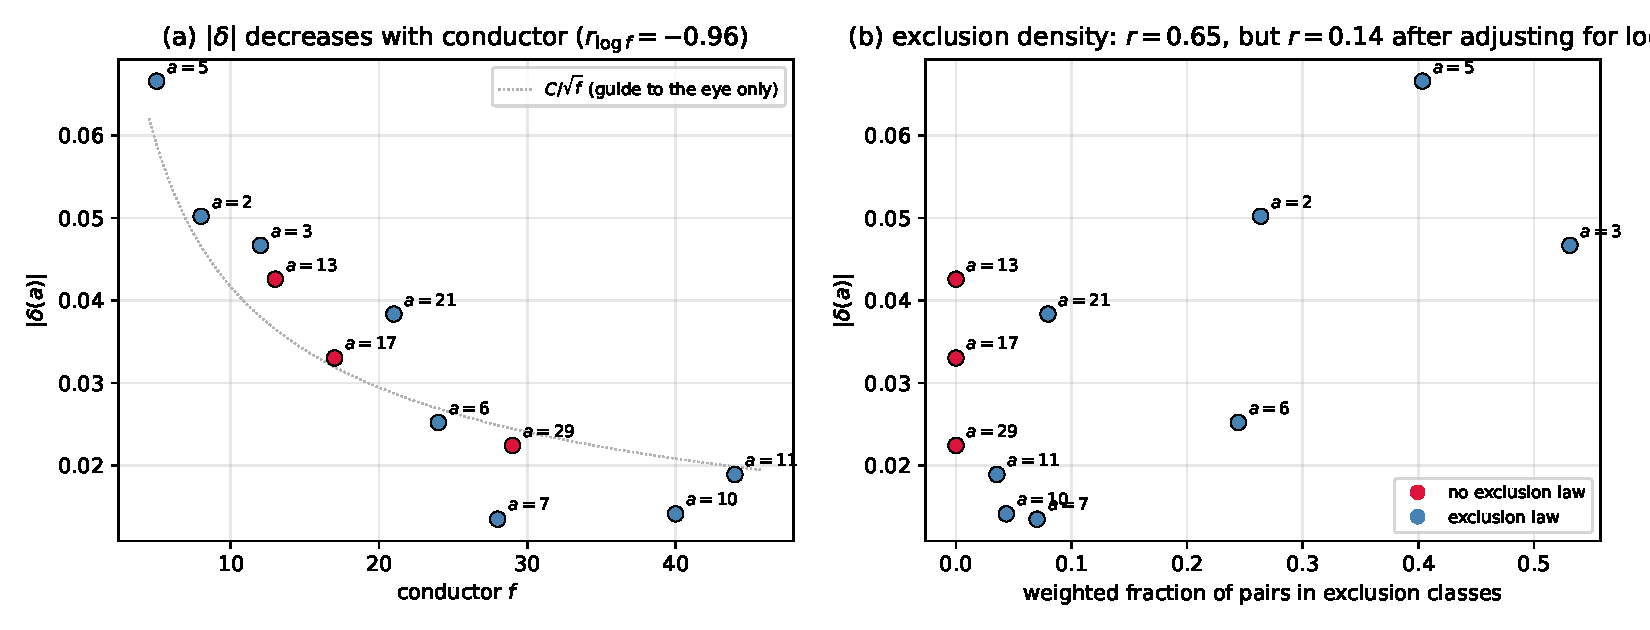
\includegraphics[width=0.98\textwidth]{fig_delta_conductor.pdf}
\caption{Left: $|\delta(a)|$ against the conductor $f$ of $\chi_a$ at
$x = 10^9$. The data points are the content of the figure; the faint dotted
curve $C/\sqrt{f}$ ($C = 0.132$) is a guide to the eye only --- as discussed
after Observation~\ref{obs:conductor}, the data do not identify an exponent and
no power law is asserted. Right: $|\delta(a)|$ against the weighted fraction of
consecutive pairs lying in exclusion classes (complete classification,
including the inadmissibility classes of base $5$). The three bases with no
exclusion classes ($a = 13, 17, 29$) are shown in red; the apparent
association in this panel is confounded with the conductor (see
Observation~\ref{obs:refutation}).}
\label{fig:conductor}
\end{figure}

We deliberately refrain from asserting an exact power law. Across the eleven
bases the products $|\delta| \cdot f$ range over $0.333$ to $0.832$, while
$|\delta| \cdot \sqrt{f}$ range over $0.0714$ to $0.1757$; the latter is the
narrower band in absolute terms, but we draw no model-selection conclusion
from that comparison, since the two products live on different scales and each
carries its own fitted multiplicative constant, so their raw widths are not
commensurable measures of fit to $|\delta|$. Neither product is constant and
neither varies monotonically with $f$. The
extremes of the $|\delta|\sqrt{f}$ band are $a = 7$ ($0.0714$) and $a = 21$
($0.1757$), a factor of $2.5$ apart, so the fitted constant $C = 0.132$ in
Figure~\ref{fig:conductor} summarises a genuinely dispersed set of values.
With eleven bases spanning $5 \le f \le 44$ we regard the evidence as
insufficient to identify an exponent. The honest statement is
Observation~\ref{obs:conductor}: a strong but imperfect monotone dependence on
$f$, whose precise shape should be derived from, rather than fitted ahead of,
a channel-by-channel analysis.

\begin{remark}
The two smallest $|\delta|$ belong to $a = 7$ and $a = 10$, with $f = 28$ and
$f = 40$; the largest to $a = 5$ with $f = 5$. As noted in
Observation~\ref{obs:conductor}, $a = 21$ with $f = 21$ sits above both
$a = 17$ ($f = 17$) and $a = 6$ ($f = 24$), so the dependence on $f$ is not
perfectly monotone --- as one would expect if the relevant quantity is a sum
over the $\varphi(f)$ channels rather than a function of $f$ alone.
\end{remark}

\section{Discussion}
\label{sec:discussion}

\subsection*{What is new here}
The ingredients are classical: the quadratic obstruction to being a primitive
root, quadratic reciprocity, the decomposition of a discriminant into prime
discriminants, and the elementary evaluation of a Jacobi-type character sum. The forbidden classes
are likewise not new: they were obtained, by a different argument and in the
fixed-shift setting, by Tinkov\'a, Waxman and
Zindulka~\cite{TinkovaWaxmanZindulka2023}, and Section~\ref{sec:twz} sets out
the overlap. What we believe this paper contributes is
(i) a derivation of the exclusion laws from a single exact counting identity
(Theorem~\ref{thm:identity}), valid for every modulus, prime or composite,
which yields the prime-conductor evaluation as a special case;
(ii) the separation of \emph{two distinct mechanisms} --- reversal, classified
completely in terms of prime discriminants
(Theorem~\ref{thm:classification}), and inadmissibility, governed by the exact
count of Theorem~\ref{thm:inadmissible}, which degenerates precisely at
$d = 5$ --- together with the \emph{converse} direction of the dichotomy
(Corollary~\ref{cor:complete}, Proposition~\ref{prop:exhaustion}), which is a
theorem here and a conjecture in~\cite{TinkovaWaxmanZindulka2023};
(iii) machine verification of the identity and two instances of the count in
Lean~4; and (iv) a cross-base measurement of the consecutive-pair Artin
correlation, in which conductor size orders the eleven measured values better
than exclusion weight does --- a statistic that does not appear in the
fixed-shift literature and that we believe to be new.

We call attention to a corrective aspect of (ii). An earlier version of this
paper classified only the reversing mechanism and asserted that base $5$
admits no exclusion law. The census prompted the re-examination --- twenty million consecutive pairs at
gaps $g \equiv 2, 3 \pmod 5$ with a zero doubly-Artin count is not a subtle
signal --- and the inadmissibility mechanism was found by asking what the
classification had missed. The refutation itself is the residue count of
Theorem~\ref{thm:inadmissible}: a zero census count, however extensive, cannot
by itself establish that an obstruction is present. That same earlier version
contained two further defects, both since corrected: the count of
Theorem~\ref{thm:inadmissible} was stated without the hypothesis
$g \not\equiv 0 \pmod d$, under which it is false and not even
integer-valued (Remark~\ref{rem:hypothesis}); and the composite case of the
dichotomy was argued by a component-wise construction that fails when a prime
factor of $d$ divides the shift (Remark~\ref{rem:oldproof}). Both are now
repaired, the first by separating the two cases and the second by replacing
the argument with the multiplicative identity of Theorem~\ref{thm:identity}.
We record the episode because it illustrates the value of exhaustive
verification against exact counts, and of machine-checking the statements most
likely to be wrong: the check of Table~\ref{tab:verification} was designed to
catch implementation errors, and instead caught a theorem-level gap.

\subsection*{Relation to earlier work}
For base $10$ the exclusion class $g \equiv 20 \pmod{40}$ and a measurement of
$\delta(10)$ were obtained by the author in earlier
work~\cite{BaldConsecutive}; the present paper
subsumes that case, since $d = 10$ gives $D = 40 = 5 \cdot 8$ and
Theorem~\ref{thm:classification} returns the single exclusion class
$g \equiv 20$.

Garcia--Kahoro--Luca~\cite{GarciaKahoroLuca2019} study primitive-root bias for
twin primes, i.e.\ the single gap $g = 2$, comparing $\varphi(p-1)$ with
$\varphi(p+1)$. It is worth being explicit that our law says nothing about
twin primes for the bases one might first consider. By
Table~\ref{tab:components}, $g = 2$ is reversing only if some component
reverses at $2$ and none is indeterminate there; the component $-4$ reverses
at $g \equiv 2 \pmod 4$ and the component $-3$ reverses at $g \not\equiv 0
\pmod 3$, but a component $q^*$ with $q \ge 5$ is indeterminate at $g = 2$,
and the component $\pm 8$ is indeterminate at $g \equiv 2 \pmod 8$. For
$d = 3$, with $f = 12$ and components $\{-3, -4\}$, both components reverse at
$g = 2$, so the count of reversing components is even and $g \equiv 2$ is
\emph{preserving}, not reversing --- as Table~\ref{tab:classification} records.
Concretely, $3$ is a primitive root of both $5$ and $7$, a twin pair at gap
$2$, so $g = 2$ is certainly not an exclusion class for base $3$, and no
reversing mechanism excludes gap $2$ for any base.

The inadmissibility mechanism, however, does. Base $5$ has conductor $5$ and
exclusion classes $g \equiv 2, 3 \pmod 5$ by
Theorem~\ref{thm:inadmissible}, and $2 \equiv 2 \pmod 5$; hence
Theorem~\ref{thm:exclusion}'s conclusion holds at gap $2$ for base $5$ by
Definition~\ref{def:exclusion}. In other words, \emph{no pair of twin primes
$p, p+2$ can have $5$ as a primitive root of both}, and the same applies to
every base with squarefree part $5$, such as $20, 45$ and $80$. We verified
this against the $3{,}804$ twin-prime pairs below $4 \times 10^5$: none has $5$
as a primitive root of both members, whereas $953$ of them have $3$ as a
primitive root of both. This appears to be the only gap-$2$ statement our
classification yields.

Pollack~\cite{Pollack2014} constructs, under GRH, infinitely many bounded-gap
prime pairs sharing a given primitive root, and
Baker--Pollack~\cite{BakerPollack2016} obtain an unconditional result for
primitive roots drawn from a large set of primes. Our results add a
base-specific constraint on where such configurations can occur: a pair
sharing the primitive root $a$ must avoid every exclusion class of $a$, and
for $a = 3$ this excludes three of the six even gap classes modulo $12$.

\subsection*{Future work}
Three directions suggest themselves. First, the channel decomposition displayed
after Observation~\ref{obs:conductor} should be carried out: a derivation from
the singular series of~\cite{HardyLittlewood1923} together with Hooley's
density computation~\cite{Hooley1967}, summed over the $\varphi(f)$ residue
channels, would replace an empirical regularity with a formula and settle the
exponent question. Second, the behaviour of $\delta(a)$ as $x$ grows should be
measured for several bases at once. Extending the present computation to
$10^{12}$ is not immediate: the implementation fixes a trial-division bound of
$10^5$, which suffices to factor $p - 1$ for $p \le 10^{10}$ but not beyond,
so a run at $10^{12}$ requires raising that bound to $10^6$, with the
corresponding increase in sieve memory and per-prime cost, and we have not
measured the resulting runtime. We therefore record it as future work rather
than as a routine extension. Third, the classification invites an analogue for
higher-order obstructions: membership in $\Art_a$ also requires $a$ to be a
non-$\ell$-th-power residue for every $\ell \mid p-1$, and the cubic case in
particular should produce exclusion laws governed by conductors of cubic
characters, with $\Q(\sqrt{-3})$ playing a distinguished role. Such an
analysis would also narrow the gap, noted in Section~\ref{sec:intro}, between
the quadratic exclusion classes classified here and the set of gap classes at
which doubly-Artin pairs genuinely fail to occur.

\section*{Acknowledgements}
The author thanks the developers of the open-source tools used in this work
(GCC, Python, \texttt{sympy}, \texttt{matplotlib}, Lean~4 and
\texttt{mathlib}).

\subsection*{Use of generative AI}
A large-language-model AI assistant was used in the preparation of this work:
for drafting and revising exposition, for writing and debugging the sieve and
analysis programs, for exploratory discussion of the classification, and for
the Lean formalisation described in Section~\ref{sec:formal}. The present
revision was also prepared with such assistance, including an adversarial
audit which located errors that are corrected here. Numerical outputs were
produced by executing deterministic programs, not synthesised by a language
model. The author is solely responsible for the content of this paper,
including any remaining errors.

\section*{Declaration of interest}
The author reports there are no competing interests to declare.

\section*{Funding}
This research received no external funding.

\section*{Data availability}
The code and results supporting this paper are available at
\url{https://github.com/jpbald93/quadratic-exclusion-laws}, a repository
dedicated to this paper. A single entry point,
\texttt{code/regenerate\_all.py}, reproduces every headline claim of this
paper from the primary contingency data and exits non-zero on any mismatch:
the dichotomy over all $72$ non-square bases $a \le 80$, the exhaustion of
Proposition~\ref{prop:exhaustion}, the $14{,}803$-case identity check, the
prime-conductor count in both cases, the twin-prime counts of
Section~\ref{sec:discussion}, and the correlations, scaled products and
incidence totals of Sections~\ref{sec:verification}--\ref{sec:delta}. Also
included are the segmented sieve and multi-base correlation program, the exact
contingency tables underlying Tables~\ref{tab:verification}
and~\ref{tab:delta}, the script reproducing Figure~\ref{fig:conductor}, and
the Lean~4 development of Section~\ref{sec:formal} with its axiom-dependency
checker. Earlier scripts implementing the superseded reversal-only classification ---
in particular they scan only even least residues, missing odd-residue classes
of odd conductors --- are \emph{not} included there; they are retained, marked
as superseded, in the author's combined repository. The computation reported here can be reproduced from the
repository on a single core; rebuilding the Lean development
additionally requires a \texttt{mathlib} binary cache.

\begin{thebibliography}{99}

\bibitem{BakerPollack2016}
R.~C. Baker and P.~Pollack,
\emph{Bounded gaps between primes with a given primitive root, II},
Forum Math. \textbf{28} (2016), no.~4, 675--687.

\bibitem{BaldConsecutive}
J.~Bald,
\emph{Correlations between primitive root statuses of consecutive primes},
preprint (2026), Zenodo,
\href{https://doi.org/10.5281/zenodo.22863946}{doi:10.5281/zenodo.22863946};
code and data at
\url{https://github.com/jpbald93/consecutive-primitive-roots}.

\bibitem{FanPollack2025}
K.~(S.)~Fan and P.~Pollack,
\emph{Counting primes with a given primitive root, uniformly},
Mathematika \textbf{71} (2025), no.~4, Paper No.~e70055.

\bibitem{GarciaKahoroLuca2019}
S.~R. Garcia, E.~Kahoro, and F.~Luca,
\emph{Primitive root bias for twin primes},
Exp. Math. \textbf{28} (2019), no.~2, 151--160.

\bibitem{GarciaLucaShiUdell2020}
S.~R. Garcia, F.~Luca, K.~Shi, and G.~Udell,
\emph{Primitive root bias for twin primes II: Schinzel-type theorems for
totient quotients and the sum-of-divisors function},
J. Number Theory \textbf{208} (2020), 400--417.

\bibitem{GuptaMurty1984}
R.~Gupta and M.~R. Murty,
\emph{A remark on Artin's conjecture},
Invent. Math. \textbf{78} (1984), no.~1, 127--130.

\bibitem{HardyLittlewood1923}
G.~H. Hardy and J.~E. Littlewood,
\emph{Some problems of `Partitio numerorum'; III: On the expression of a
number as a sum of primes},
Acta Math. \textbf{44} (1923), 1--70.

\bibitem{HeathBrown1986}
D.~R. Heath-Brown,
\emph{Artin's conjecture for primitive roots},
Quart. J. Math. Oxford Ser. (2) \textbf{37} (1986), no.~145, 27--38.

\bibitem{Hooley1967}
C.~Hooley,
\emph{On Artin's conjecture},
J. Reine Angew. Math. \textbf{225} (1967), 209--220.

\bibitem{JarviniemiPeruccaSgobba2025}
O.~J\"arviniemi, A.~Perucca, and P.~Sgobba,
\emph{Unified treatment of Artin-type problems II},
Res. Number Theory \textbf{11} (2025), no.~42, 19~pp.

\bibitem{Kimmel2024}
N.~Kimmel,
\emph{Artin's primitive root conjecture in number fields and for matrices},
Acta Arith. \textbf{216} (2024), no.~4, 329--348.

\bibitem{LOS2016}
R.~J. Lemke~Oliver and K.~Soundararajan,
\emph{Unexpected biases in the distribution of consecutive primes},
Proc. Natl. Acad. Sci. USA \textbf{113} (2016), no.~31, E4446--E4454.

\bibitem{Moree2012}
P.~Moree,
\emph{Artin's primitive root conjecture --- a survey},
Integers \textbf{12A} (2012), Article A13, 100~pp.

\bibitem{PeruccaShparlinski2025}
A.~Perucca and I.~E. Shparlinski,
\emph{Uniform bounds for the density in Artin's conjecture on primitive roots},
Bull. Lond. Math. Soc. \textbf{57} (2025), 978--991.

\bibitem{TinkovaWaxmanZindulka2023}
M.~Tinkov\'a, E.~Waxman, and M.~Zindulka,
\emph{Artin twin primes},
J. Number Theory \textbf{247} (2023), 274--304;
\texttt{arXiv:2010.15988}.

\bibitem{Pollack2014}
P.~Pollack,
\emph{Bounded gaps between primes with a given primitive root},
Algebra Number Theory \textbf{8} (2014), no.~7, 1769--1786.

\end{thebibliography}

\end{document}
